\chapter{Convolutional Neural Networks}
\label{ch:cnn}
Convolutional Neural Networks have been around for some time, but gained popularity mostly in the recent years, since better hardware was available. It is a deep learning algorithm, mostly used on images. The tasks CNNs can solve include image classification or image segmentation and many others. Nowadays they are widely used for medical imaging problems. 

They were first introduced by Yann LeCun et al. in 1999 \cite{lecun1999}. They used CNN for recognising handwritten numbers. This classic dataset is known as MNIST. Underlying principles of convolutional neural networks are inspired by the visual system of cats - discovery of neurons responsive to different stimuli in different regions (receptive fields), which are then put together.

CNN is able to detect low-level features (for example edges) to high-level features (whole objects) in images. They are detected by applying appropriate filters. These filters are not pre-defined, but rather gained from training the network. To understand how this works, we need to introduce two important operations: convolution and pooling.

\textbf{Convolution} can be described as multiplication followed by summation. This operation is explained by the image \ref{fig:convolution-image}. Input for convolution is an image \textit{I}. Then we take a filter (or kernel) \textit{K} - which is a matrix of weights - and slide it through the image, computing convolutions for every position of the filter. Result \textit{I * K} is called a feature map. You can see the resulting feature map has smaller resolution than the original image. If we want to keep the original resolution, we can pad the original image around its edges. These filters are responsible for detecting features in images. CNNs usually do not consist of only one convolutional layer, so it is possible to detect high-level features. 

Another matrix operation is \textbf{pooling} (in \cite{lecun1999} originally referred to as sub-sampling). It is applied to feature maps from the previous convolutional layer. They down-sample (lower resolution of) feature maps, in order to reduce computation time, but also to allow for extracting more high-level features. There are two types of pooling, max and average pooling. Again, a filter passes through a feature map and returns the maximum and average respectively from its receptive field. This operation is visualised in \ref{fig:pooling-image}. In this image, stride of 2 was used. It means the filter did not pass the image pixel by pixel, but in ``steps'' of two.

\begin{figure}[ht]
    \centering
    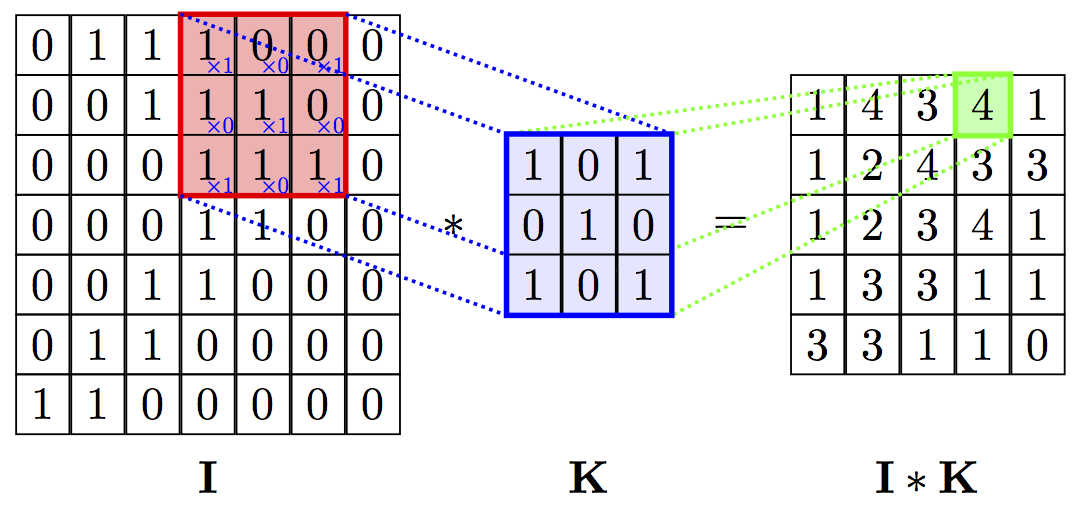
\includegraphics[width=200pt]{images/convolution-image.png}
    \caption{Visualisation of convolution}
    \label{fig:convolution-image}
\end{figure}

\begin{figure}[ht]
    \centering
    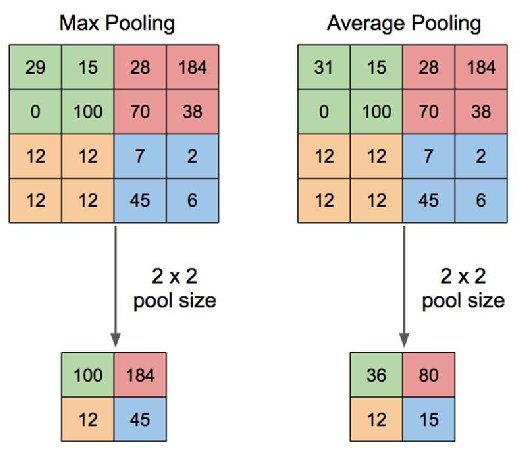
\includegraphics[width=200pt]{images/pooling.jpg}
    \caption{Visualisation of pooling}
    \label{fig:pooling-image}
\end{figure}

To see and understand how these layers work together, we can look at popular AlexNet \cite{alexnet2012} and its architecture \ref{fig:alexnet}. AlexNet won ImageNet classification competition in 2012, introducing an architecture which achieved a top-5 error of 15.3\%, which was 10\% lower than the second place.

Alex Krizhevsky used images of the volume of 224 x 224 x 3 (channels for RGB). These are fed to the first convolutional layer with 96 kernels of size 11 x 11 x 3. Every kernel produces one feature map, so the result is 55 x 55 x 96, which is then max-pooled and fed to the second convolutional layer. The second convolutional layer consists of 256 kernels of size 5 x 5 x 96, producing volume of 27 x 27 x 256, which is max-pooled again. The third layer contains 384 kernels of 3 x 3 x 256. Outputs (without max pooling) are sent to the fourth layer with 384 kernels of 3 x 3 x 384 and then to the fifth layer with 256 kernels of 3 x 3 x 384. Then two fully connected layers follow.

\begin{figure}[ht]
    \centering
    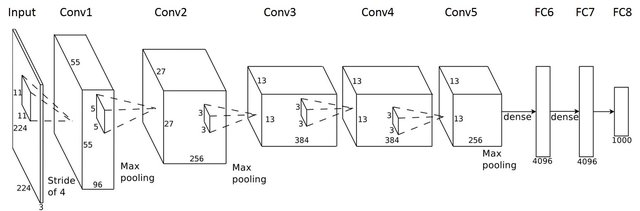
\includegraphics{images/alex-net.jpg}
    \caption[Architecture of AlexNet]{Architecture of AlexNet \cite{alexnet2012}}
    \label{fig:alexnet}
\end{figure}

Since 2012, CNNs have become very popular. There have been many extentions made to either solve problems occuring with CNNs or expand their use. I will talk about some of them next.

%----SECTIONS----%
\section{UNet}
The typical use of CNNs was mainly classification. The original architectures would usually just recognise what is on the image, but not where - which is the point of segmentation. In 2015, a new type of network for segmentation of biomedical images Unet was introduced \cite{unet2015}.

It is a FCV - fully convolutional network. That means there are no dense layers, only convolutions. This architecture (\ref{fig:unet}) consists of two parts or paths - \textbf{encoder} and \textbf{decoder}, which resembles the letter U. Hence, the name U-Net. Encoder serves for down sampling the high-resolution input image to a low-resolution output to find out what is in the image. Decoder up samples the low-resolution image back to the original resolution, retrieving locations of the features.

\begin{figure}[ht!]
    \centering
    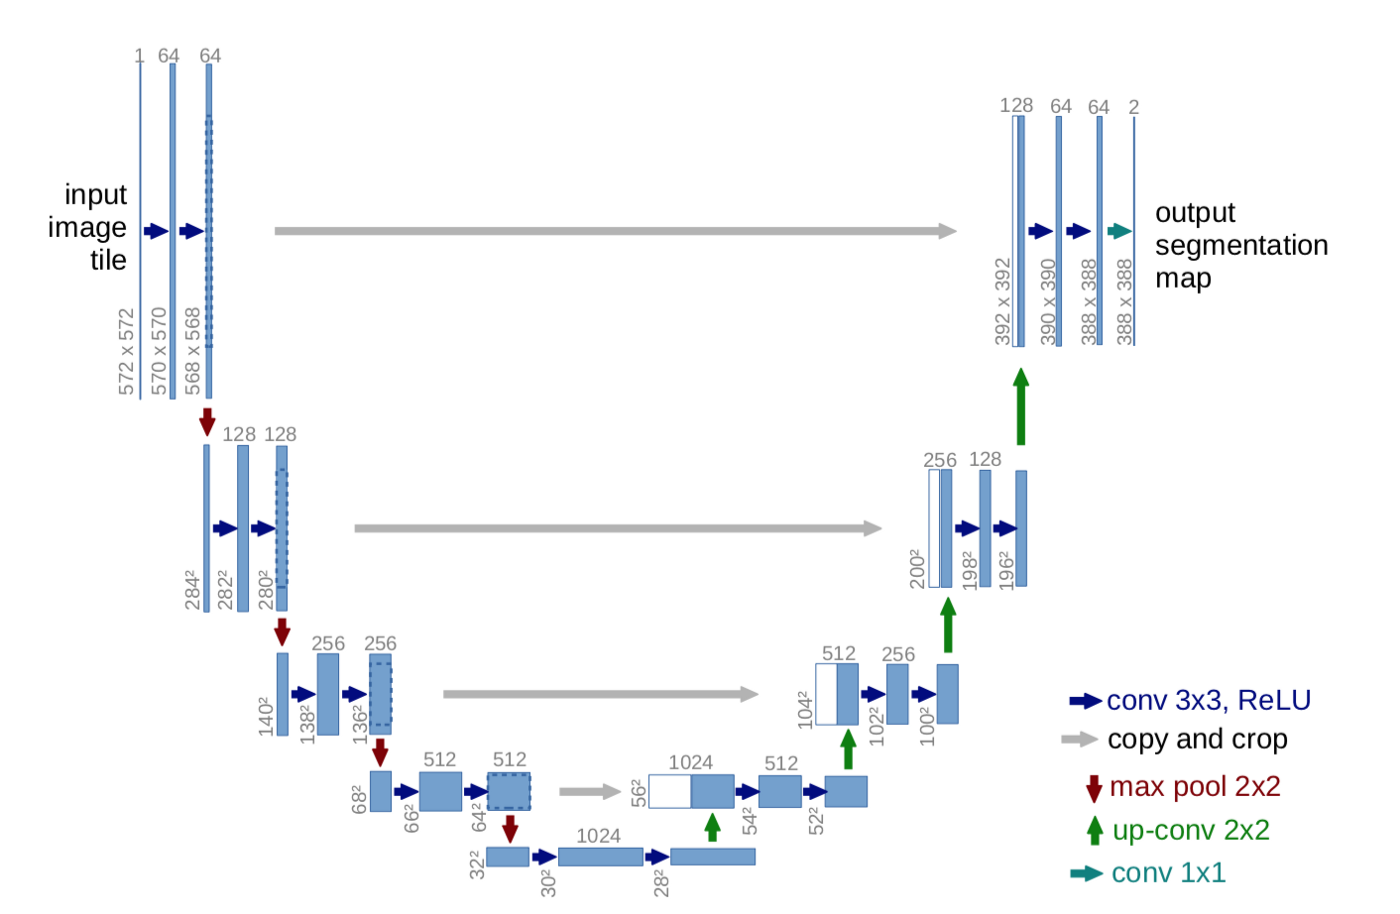
\includegraphics[width=300pt]{images/unet.png}
    \caption[Architecture of UNet]{Architecture of UNet \cite{unet2015}}
    \label{fig:unet}
\end{figure}

Encoder is a typical CNN, consisting of 3 blocks containing 2 convolutional layers followed by a max-pooling layer.

Decoder is more interesting. It is symmetrical to the encoder - 3 block consisting of up-convolution (transposed convolution) and 2 convolutions. The output is a predicted segmentation mask. Transposed convolution can be viewed as an operation opposite to convolution (but it is not the most precise definition). It creates a higher-resolution image from a low-resolution image. Furthermore, every result of up-convolution is concatenated with the feature map from the corresponding level in the encoder through skip connections. UNet has proven to perform very well on biomedical images.  

\pagebreak
\section{ResNet}
Another expansion built on CNNs is ResNet (Residual Network) \cite{resnet2016}, which succeeded in tackling issues with very deep networks. The general consensus was, the deeper the network is, the better performance it gives. However, it was observed, that training error for deeper networks gets higher than for their less deep counterparts. 

The degradation problem is caused by vanishing/exploding gradients. During backpropagation, multiplication of small (<1) and big (>1) numbers occurs. In deep networks, the multiplication takes place many times, causing it to get smaller and smaller until it vanishes or bigger and bigger until it blows up.

This problem can be solved by introducing residual blocks \ref{fig:res-block}. A skip connection is used to allow \textit{x} to be added to the output of later layers. This means, if vanishing gradient occurs, the network can be saved by ``going back'' to the previous layers. \ref{fig:resnet} shows a plain network and its counterpart (ResNet) with skip connections.

\begin{figure}[ht!]
    \centering
    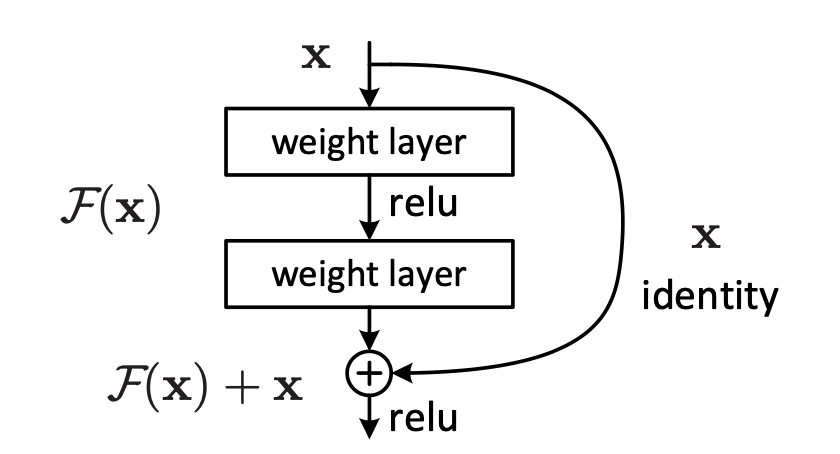
\includegraphics[width=130pt]{images/residual-block.png}
    \caption[Residual block]{Residual block \cite{resnet2016}}
    \label{fig:res-block}
\end{figure}

\begin{figure}[ht!]
    \centering
    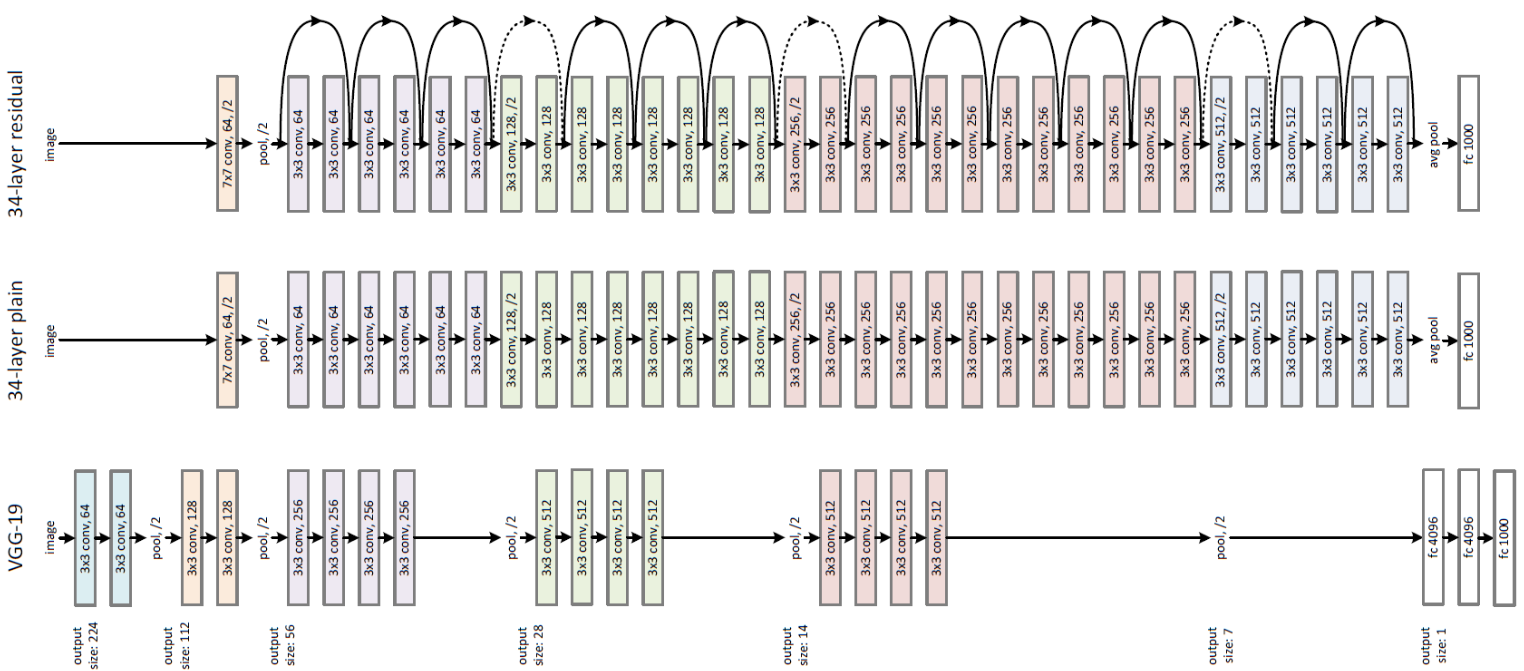
\includegraphics[width=350pt]{images/resnet.png}
    \caption[ResNet architecture]{ 34 layer ResNet (top), 34 layer plain network (middle), 19 layer VGG-19 (bottom)\cite{resnet2016}}
    \label{fig:resnet}
\end{figure}

\pagebreak
\section{DenseNet}
DenseNet \cite{densenet2017} was introduced in 2017. In an architecutre of this type, each layer receives ouputs from all the previous layers and then passes its input to all subsequent layers, to ensure maximum information flow.  In contrast to ResNet, where outputs are combined through summation, DenseNet uses concatenation.

Its name comes from the dense connectivity between layers. Suppose we have \textit{L} layers in the architecture. \textit{$l^{th}$} layer takes \textit{$l^{th}$} inputs (feature maps from previous layers) and its output goes to \textit{L} - \textit{$l^{th}$} following layers. This is illustrated in Figure \ref{fig:densenet}.

One of the improvements DenseNet brought, was a smaller amount of parameters to train, compared to traditional architectures or even ResNet. This feature makes it more computationally efficient. Dense layers have a few filters, which means, that the ``total'' number of feature maps passed through the network is rather small. The network then makes a decision based on all feature maps that appeared in it. Other advantages of DenseNets include memory efficiency. Furthermore, dense connections were observed to help with overfitting on small data sets.


\begin{figure}[ht!]
    \centering
    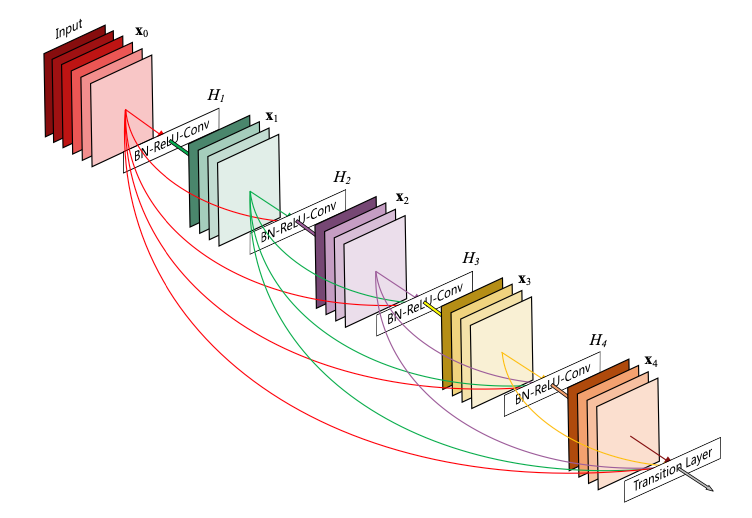
\includegraphics[width=200pt]{images/densenet.png}
    \caption[DenseNet architecture]{DenseNet architecture \cite{densenet2017}}
    \label{fig:densenet}
\end{figure}

\pagebreak
\section{R-CNN, Fast R-CNN, Faster R-CNN}
Previous architectures I was talking about served for solving classification (AlexNet, DenseNet, ResNet) or segmentation tasks (UNet). Another computer vision problem is object detection - finding instances of objects of classes in an image. That means localizing several objects of several classes withing one image.

R-CNN \cite{rcnn2014} (R stands for regions) proposed a method which combines region proposals and CNNs. Region proposals are a set of ``sub-images'' for classification. These regions are chosen by selective search. R-CNN architecture consists of 3 modules \ref{fig:rcnn}: First module takes the input image and generates around 2000 region proposals. These are then fed to a CNN which computes feature maps for them. And the last module is a linear SVM, which classifies the regions.

\begin{figure}[ht!]
    \centering
    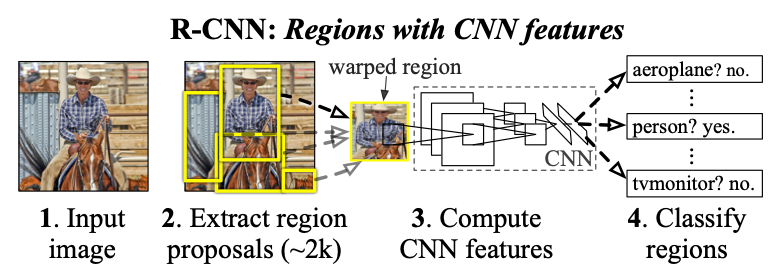
\includegraphics[width=200pt]{images/r-cnn.png}
    \caption[R-CNN modules]{R-CNN modules \cite{rcnn2014}}
    \label{fig:rcnn}
\end{figure}

The problem with R-CNN is that it is slow. This problem stems from the use of selective search to produce proposals, which are processed by CNN one by one . Therefore, its author came up with another method to speed up the process, Fast R-CNN \cite{fast-rcnn2015}. Input for this network is the whole image and a set of proposals. Generated convolutional maps are passed to the ROI (region of interest) pooling layer. This layer resizes them to a fixed size, so they can be fed into a fully connected layer. Squeezing an image and its proposals together reduces the number of convolutional passes and makes the whole process faster. 

Even faster version called Faster R-CNN was developed \cite{faster-rcnn2017}. Instead of using selective search to exhaustively produce region proposals, a Region Proposal Network is introduced. It is a fully convolutional network, which takes an image of any size as its input and outputs predictded object bounds. Those are then passed to the ROI pooling layer and then classified. 
\section{Capsule Network}
CNNs classify objects based on features they find in the image. When it spots a head, arms, legs and a body, it will classify the image as a person. However, spatial relationship between the features or their rotation is not considered. 

CapsNet \cite{capsnet2017} was developed to address this problem. A new neuron organisation called \textit{capsule} is proposed. Capsules are groups of neurons within one layer. Capsules output vectors (not scalars!), because they can encode more information. The size of the vector indicates the probability of the feature to even exist and its orientation describes various properties, like size, rotation, position, texture, etc. 

The proposed architecture (Fig \ref{fig:capsnet}) is quite simple. The first layer is convolutional and extracts features for capsules. The second layer is Primary Capsule layer. Consists of 32 capsules of 8 kernels and outputs 8D vectors. Those go to Digit Capsule Layer. This layer consists of 10 capsules (one capsule per class, in this case digits). All the capsules from the lower (primary) layer send their output to all the capsules in the higher (digit) level. The higher level outputs 16D vectors, which are fed to 3 fully connected layers. 

Dynamic routing is a process between two capsule layers. Its job is to replace max-pooling, during which spatial information is lost. Thanks to dynamic routing, output of one capsule gets send to the most appropriate parent capsule in the higher level. 

\begin{figure}[ht!]
    \centering
    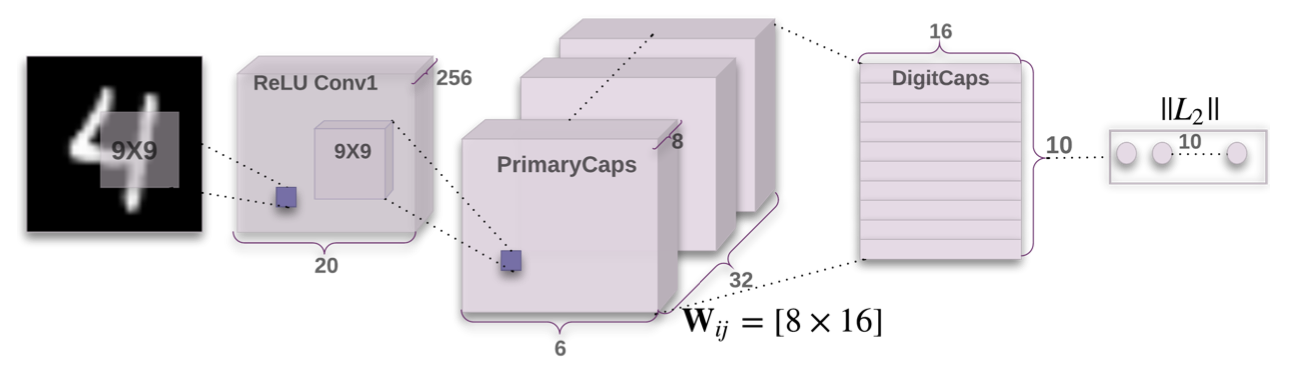
\includegraphics[width=300pt]{images/capsnet.png}
    \caption[CapsuleNetwork architecture]{CapsuleNetwork architecture \cite{capsnet2017}}
    \label{fig:capsnet}
\end{figure}

The model achieves very good results on classifying digits from MNIST and can also recognise overlapped digits in the MultiMNIST dataset. The way Capsule Networks work resembles human brain more than conventional CNNs. Even though they proved themselves successful on simple tasks like digit recognition, CapsuleNetworks are still a subject of research and need to improve their performance on more complex tasks. 




